% are-self Whitepaper (Technical Edition)
% Packages: geometry, amsmath, amssymb, booktabs, graphicx, hyperref, url, listings, tikz
% Compilation: pdflatex are_self_whitepaper.tex

\documentclass[11pt]{article}

\usepackage[margin=1in]{geometry}
\usepackage{amsmath,amssymb}
\usepackage{booktabs}
\usepackage{array}
\usepackage{graphicx}
\usepackage{hyperref}
\usepackage{url}
\usepackage{listings}
\usepackage{tikz}
\usetikzlibrary{shapes.geometric, arrows.meta, positioning, fit}

\lstset{
	basicstyle=\ttfamily\small,
	breaklines=true,
	frame=single,
	numbers=left,
	numberstyle=\tiny,
	keywordstyle=\bfseries,
	commentstyle=\itshape,
	showstringspaces=false,
}

\hypersetup{
	pdftitle={are-self: A Unified Platform for Orchestration and Autonomous Reasoning},
	pdfauthor={Talos Project},
	colorlinks=true,
	linkcolor=blue,
	citecolor=blue,
	urlcolor=blue
}

\title{are-self: A Unified Platform for Orchestration and Autonomous Reasoning}
\author{Talos Project}
\date{\today}

\begin{document}
	\sloppy
	\maketitle

	% -------------------------------------------------------------------------
	% 1. EXECUTIVE SUMMARY
	% -------------------------------------------------------------------------
	\begin{abstract}
		are-self is an AI-assisted automation platform that unifies two traditionally separate domains: graph-based workflow orchestration and identity-driven autonomous reasoning. Built on the Talos Django control plane, it addresses the industry pain of fragmented automation tools by providing a single system where build pipelines, remote agent execution, and AI reasoning run as first-class citizens of the same graph vocabulary. The platform delivers persistent, typed state for full audit trails and recovery; a formal transition semantics for labeled directed graphs; and a cognition stack with focus/XP economy, vector memory, and a work-eligibility gatekeeper that prevents spinning up AI workers without actionable work. This whitepaper provides exhaustive technical detail for lead developers, data scientists, and machine learning engineers: architecture diagrams, methodology breakdowns, code snippets from the live codebase, and verified implementation parameters.
	\end{abstract}

	% -------------------------------------------------------------------------
	% 2. PROBLEM STATEMENT
	% -------------------------------------------------------------------------
	\section{Problem Statement}
	\label{sec:problem}

	The development of AI-assisted automation has reached a critical juncture: orchestration and cognition are typically implemented as separate systems, leading to fragmented workflows, lost context, and inefficient resource use.

	\subsection{Orchestration and Cognition as Separate Concerns}
	Traditional automation platforms treat workflow orchestration (launching builds, running scripts, distributing work across agents) and AI reasoning (LLM turn loops, tool use, memory) as distinct domains. This split forces engineers to glue together disparate tools, lose execution context when crossing boundaries, and accept that AI workers cannot natively participate in the same graph that drives process execution. The result is brittle pipelines, manual handoffs, and systems that cannot recover gracefully when AI sessions fail or time out \cite{talosLiveCodebase}.

	\subsection{The Need for Persistent, Typed State}
	Many orchestration systems rely on transient in-memory state. When a process crashes, a network partition occurs, or a Celery worker restarts, execution context is lost. Audit trails are incomplete, and recovery requires manual intervention. In AI-assisted workflows, this is especially problematic: a reasoning session that has consumed dozens of turns and tool calls cannot be resumed if its state was never persisted. The industry needs systems where almost every important runtime decision is driven by database rows, enabling inspectable state, full audit trails, and recovery from failures without losing execution context \cite{talosLiveCodebase}.

	\subsection{Scaling and Resource Efficiency}
	Distributed execution across local and remote agents introduces complexity: discovery, health checks, log streaming, and failure handling must be unified. AI workers, meanwhile, consume significant compute; spinning up sessions when no actionable work exists wastes resources and increases cost. Systems need a work-eligibility gatekeeper that decides \emph{whether} an AI should work before creating a session, and a scheduler that decides \emph{when} it could work---avoiding idle cognition and ensuring agents only run when they have real tasks \cite{talosTemporal,talosPFC}.

	% -------------------------------------------------------------------------
	% 3. THE SOLUTION & ARCHITECTURE
	% -------------------------------------------------------------------------
	\section{The Solution \& Architecture}
	\label{sec:solution}

	are-self is implemented by Talos, a Django control plane that couples a graph-based orchestration engine with an autonomous reasoning engine. Both halves share the same vocabulary: a reasoning run is another kind of spike execution, invoked via the native handler \texttt{run\_frontal\_lobe}. The system is built around persistent, typed state and a brain-themed modular decomposition.

	\subsection{System Design Overview}
	The architecture has two pillars: (i) \emph{Orchestration}---the Central Nervous System (CNS) graph engine, Peripheral Nervous System (PNS) agent discovery and execution, and environments for context---and (ii) \emph{Cognition}---frontal lobe (reasoning), parietal lobe (tools), hippocampus (memory), temporal lobe (scheduling), prefrontal cortex (work allocation), and identity (persona). The CNS connects to PNS and environments; the CNS invokes frontal lobe and temporal lobe; the frontal lobe connects to parietal lobe, hippocampus, and identity; the temporal lobe connects to prefrontal cortex; and the prefrontal cortex invokes the frontal lobe when work exists \cite{talosCombined,talosLiveCodebase}.

	\subsection{Request Path and URL Routing}
	The live runtime uses the \texttt{central\_nervous\_system} stack registered in \texttt{config/settings.py} and routed from \texttt{config/urls.py}. The active request path is \cite{talosLiveCodebase}:

	\begin{lstlisting}[language=Python, caption={URL routing and API registration (config/urls.py).}]
urlpatterns = [
    path("", include("dashboard.urls")),
    path("central_nervous_system/", include("central_nervous_system.urls.urls")),
    path("environments/", include("environments.urls")),
    path("reasoning/", include("frontal_lobe.urls")),
    path("api/v1/", include(v1_router.urls)),
    path("api/v2/", include(V2_ROUTER.urls)),
    path("admin/", admin.site.urls),
    path("api-auth/", include("rest_framework.urls", namespace="rest_framework")),
    path("mcp/", include("djangorestframework_mcp.urls")),
]
	\end{lstlisting}

	V2 routers extend CNS, Temporal Lobe, Identity, Prefrontal Cortex, Hippocampus, Reasoning, Parietal Lobe, and PNS. Note: there are two distinct ``MCP'' concepts---external \texttt{djangorestframework\_mcp} at \texttt{/mcp/} (DRF viewsets) and internal \texttt{ParietalMCP.execute()} which dynamically loads \texttt{mcp\_*} tool modules for the LLM~\cite{talosLiveCodebase}.

	\subsection{Architecture Diagram: High-Level Data Flow}
	\begin{figure}[ht]
		\centering
		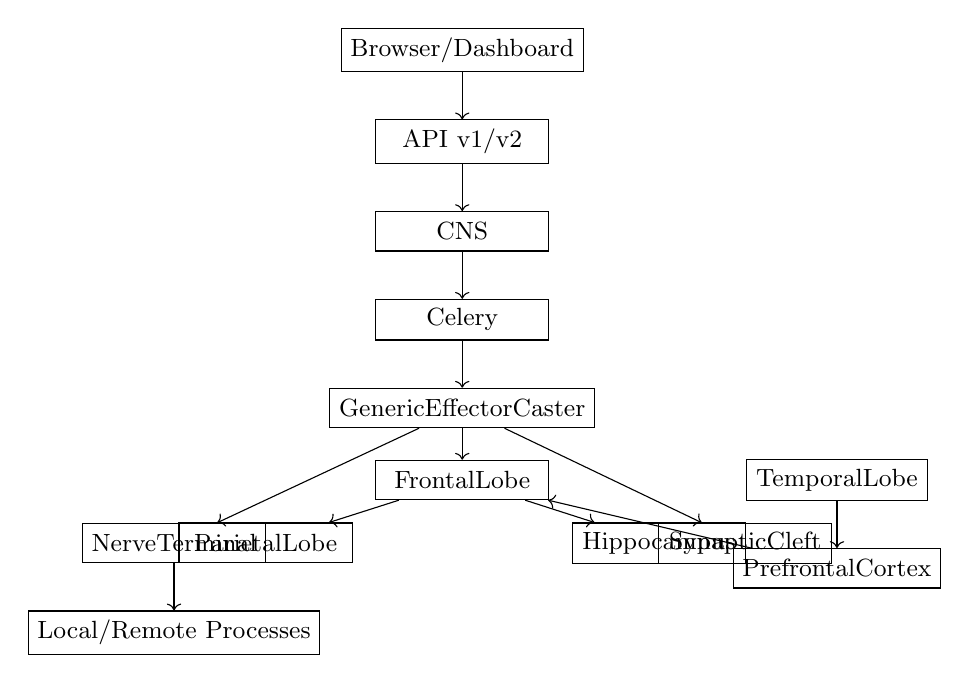
\begin{tikzpicture}[
			node distance=0.6cm,
			box/.style={rectangle, draw, minimum width=2.2cm, minimum height=0.5cm, font=\small},
			subbox/.style={rectangle, draw, dashed, inner sep=4pt}
			]
			\node[box] (browser) {Browser/Dashboard};
			\node[box, below=of browser] (api) {API v1/v2};
			\node[box, below=of api] (cns) {CNS};
			\node[box, below=of cns] (celery) {Celery};
			\node[box, below=of celery] (caster) {GenericEffectorCaster};
			\node[box, below left=1.2cm and 0.8cm of caster] (nt) {NerveTerminal};
			\node[box, below=0.4cm of caster] (fl) {FrontalLobe};
			\node[box, below right=1.2cm and 0.8cm of caster] (sc) {SynapticCleft};
			\node[box, below=of nt] (proc) {Local/Remote Processes};
			\node[box, below left=0.4cm of fl] (pl) {ParietalLobe};
			\node[box, below right=0.4cm of fl] (hippo) {Hippocampus};
			\node[box, right=2.5cm of fl] (tl) {TemporalLobe};
			\node[box, below=of tl] (pfc) {PrefrontalCortex};
			\draw[->] (browser) -- (api);
			\draw[->] (api) -- (cns);
			\draw[->] (cns) -- (celery);
			\draw[->] (celery) -- (caster);
			\draw[->] (caster) -- (nt);
			\draw[->] (caster) -- (fl);
			\draw[->] (caster) -- (sc);
			\draw[->] (nt) -- (proc);
			\draw[->] (fl) -- (pl);
			\draw[->] (fl) -- (hippo);
			\draw[->] (tl) -- (pfc);
			\draw[->] (pfc) -- (fl);
		\end{tikzpicture}
		\caption{High-level data flow: CNS routes through Celery to GenericEffectorCaster, which dispatches to NerveTerminal (processes), FrontalLobe (reasoning), or SynapticCleft (events). TemporalLobe $\to$ PrefrontalCortex $\to$ FrontalLobe when work exists.}
		\label{fig:arch-high}
	\end{figure}

	\subsection{Cross-Module Architecture (Orchestration and Cognition)}
	\begin{figure}[ht]
		\centering
		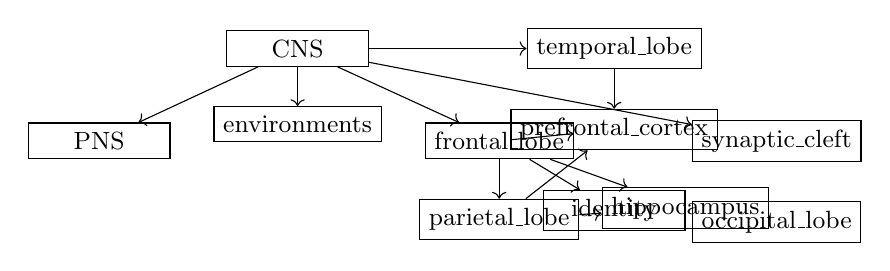
\begin{tikzpicture}[
			node distance=0.5cm,
			box/.style={rectangle, draw, minimum width=1.8cm, font=\small}
			]
			\node[box] (cns) {CNS};
			\node[box, below left=1cm of cns] (pns) {PNS};
			\node[box, below=of cns] (env) {environments};
			\node[box, below right=1cm of cns] (fl) {frontal\_lobe};
			\node[box, right=2cm of cns] (tl) {temporal\_lobe};
			\node[box, below=of tl] (pfc) {prefrontal\_cortex};
			\node[box, below=of fl] (pl) {parietal\_lobe};
			\node[box, below right=0.5cm of fl] (hippo) {hippocampus};
			\node[box, below=of pfc] (identity) {identity};
			\node[box, right=1.5cm of fl] (sc) {synaptic\_cleft};
			\node[box, below=of sc] (ol) {occipital\_lobe};
			\draw[->] (cns) -- (pns);
			\draw[->] (cns) -- (env);
			\draw[->] (cns) -- (fl);
			\draw[->] (cns) -- (tl);
			\draw[->] (cns) -- (sc);
			\draw[->] (fl) -- (pl);
			\draw[->] (fl) -- (hippo);
			\draw[->] (fl) -- (identity);
			\draw[->] (tl) -- (pfc);
			\draw[->] (pfc) -- (fl);
			\draw[->] (pl) -- (hippo);
			\draw[->] (pl) -- (pfc);
		\end{tikzpicture}
		\caption{Cross-module architecture from \texttt{docs/doc-generator/combined\_\_documentation.md}.}
		\label{fig:cross-module}
	\end{figure}

	\subsection{Graph Vocabulary and Mathematical Model}
	The static graph is \cite{talosCNS,talosCombined,talosLiveCodebase}:
	\begin{itemize}
		\item \textbf{NeuralPathway:} the protocol or graph container.
		\item \textbf{Neuron:} a node in that graph.
		\item \textbf{Axon:} a directed edge between two neurons, labeled as \texttt{flow}, \texttt{success}, or \texttt{failure}.
		\item \textbf{Effector:} a configured action bound to a \texttt{TalosExecutable}, argument assignments, switches, and a distribution mode.
	\end{itemize}

	The runtime graph is:
	\begin{itemize}
		\item \textbf{SpikeTrain:} one execution of a \texttt{NeuralPathway}.
		\item \textbf{Spike:} one execution of one \texttt{Neuron}/\texttt{Effector} within that \texttt{SpikeTrain}.
		\item \textbf{provenance:} the parent \texttt{Spike} that caused a later \texttt{Spike} to exist.
		\item \textbf{blackboard:} JSON working memory carried along execution branches.
	\end{itemize}

	Mathematically, the static graph is $G = (V, E, \lambda)$ where $V = \{\text{Neuron}\}$, $E \subseteq V \times V$, and $\lambda(e) \in \{\text{flow}, \text{success}, \text{failure}\}$. The runtime is an unfolding execution tree over time, not a simple replay of $G$ \cite{talosCNS,talosLiveCodebase}.

	\subsection{Transition Rule and Wave Dispatch}
	For finished spike $s$ with $\sigma(s) \in \{\text{SUCCESS}, \text{FAILED}\}$ \cite{talosCNS,talosCombined}:
	$$
	L_{\text{enabled}}(s) = \{\text{flow}\} \cup \begin{cases}
	\{\text{success}\} & \sigma(s) = \text{SUCCESS} \\
	\{\text{failure}\} & \sigma(s) = \text{FAILED}
	\end{cases}
	$$
	For each $e = (\nu(s), v)$ with $\lambda(e) \in L_{\text{enabled}}(s)$: create spike at $v$. The \texttt{cast\_cns\_spell} Celery task executes one spike; in \texttt{finally}, it always calls \texttt{check\_next\_wave}, making the engine self-driving.

	\subsubsection{Implementation: dispatch\_next\_wave}
	The core dispatch logic from \texttt{central\_nervous\_system/central\_nervous\_system.py} \cite{talosLiveCodebase}:

	\begin{lstlisting}[language=Python, caption={Wave dispatch logic (simplified).}]
def dispatch_next_wave(self) -> None:
    with transaction.atomic():
        self.spike_train.refresh_from_db()
        if self.spike_train.status_id == SpikeTrainStatus.STOPPING:
            self._finalize_spawn_unsafe()
            return
        spikes = self.spike_train.spikes.select_for_update().all()
        if not spikes.exists():
            self._dispatch_graph_roots()
            return
        finished_spikes = spikes.filter(
            status_id__in=[SpikeStatus.SUCCESS, SpikeStatus.FAILED]
        )
        parents_with_children = Spike.objects.filter(
            spike_train=self.spike_train, provenance__isnull=False
        ).values_list("provenance_id", flat=True)
        for spike in finished_spikes:
            if spike.id in parents_with_children:
                continue
            self._process_graph_triggers(spike)
        self._finalize_spawn_unsafe()

def _process_graph_triggers(self, finished_spike: Spike) -> None:
    valid_wire_types = [AxonType.TYPE_FLOW]
    if finished_spike.status_id == SpikeStatus.SUCCESS:
        valid_wire_types.append(AxonType.TYPE_SUCCESS)
    elif finished_spike.status_id == SpikeStatus.FAILED:
        valid_wire_types.append(AxonType.TYPE_FAILURE)
    axons = Axon.objects.filter(
        pathway=self.spike_train.pathway,
        source=finished_spike.neuron,
        type_id__in=valid_wire_types,
    )
    for wire in axons:
        self._create_spike_from_node(
            neuron=wire.target, provenance=finished_spike
        )
	\end{lstlisting}

	\subsubsection{Self-Driving Loop: cast\_cns\_spell}
	\begin{lstlisting}[language=Python, caption={Celery task \texttt{cast\_cns\_spell} (central\_nervous\_system/tasks.py).}]
@shared_task(bind=True)
def cast_cns_spell(self, spike_id):
    spike_train_id = None
    try:
        spike = Spike.objects.only("spike_train_id").get(id=spike_id)
        spike_train_id = spike.spike_train_id
        spike.celery_task_id = self.request.id
        spike.save(update_fields=["celery_task_id"])
        caster = GenericEffectorCaster(spike_id=spike_id)
        caster.execute()
    except Exception as e:
        spike = Spike.objects.get(id=spike_id)
        spike.status_id = SpikeStatus.FAILED
        spike.execution_log += f"\n[CELERY FATAL] Task crashed: {e}\n"
        spike.save(update_fields=["status", "execution_log"])
        raise e
    finally:
        if spike_train_id:
            transaction.on_commit(lambda: check_next_wave.delay(spike_train_id))
	\end{lstlisting}

	The \texttt{finally} block ensures the next wave is always triggered; that is the self-driving property \cite{talosLiveCodebase}.

	\subsection{Context Resolution Precedence}
	Context composition: $C = \text{metadata} \oplus \text{env} \oplus \text{blackboard} \oplus \text{effector} \oplus \text{neuron}$. Precedence (rightmost wins): neuron $>$ effector $>$ blackboard $>$ env $>$ metadata \cite{talosCNS,talosCombined}. The implementation in \texttt{resolve\_environment\_context} applies: metadata/base objects, then environment variables, then blackboard, then effector defaults, then neuron overrides \cite{talosLiveCodebase}.

	\subsection{Distribution Modes}
	After spike creation, cardinality is chosen \cite{talosCNS,talosCombined}:
	\begin{itemize}
		\item \texttt{LOCAL\_SERVER}: one spike, no remote target.
		\item \texttt{ONE\_AVAILABLE\_AGENT}: one spike, first online \texttt{NerveTerminalRegistry} by \texttt{last\_seen}.
		\item \texttt{ALL\_ONLINE\_AGENTS}: clone one spike per online agent.
		\item \texttt{SPECIFIC\_TARGETS}: clone one spike per pinned \texttt{EffectorTarget}.
	\end{itemize}

	\subsection{Cognition Engine: Session Model and Turn Loop}
	The cognitive runtime is centered on \texttt{ReasoningSession}, \texttt{ReasoningTurn}, \texttt{ChatMessage}, \texttt{SessionConclusion}, \texttt{ToolDefinition}/\texttt{ToolCall}, and \texttt{TalosEngram}. A \texttt{ReasoningSession} is linked to its originating \texttt{Spike} and optionally to \texttt{IterationShiftParticipant}. \texttt{IdentityDisc} provides persona, enabled tools, and model~\cite{talosLiveCodebase}.

	Each turn assembles from: (1) system identity prompt, (2) L1/L2 history cache, (3) volatile addon messages, (4) sensory trigger (engram catalog). L1: last 2 turns full; L2: older turns with truncated tool results and pruned monologue \cite{talosFrontal,talosLiveCodebase}.

	\subsection{Session Economy (Frontal Lobe)}
	\cite{talosCombined,talosFrontal}
	$$
	\text{current\_level} = \lfloor \text{total\_xp} / 100 \rfloor + 1, \quad
	\text{max\_focus} = 10 + \lfloor (\text{current\_level} - 1) \cdot 0.5 \rfloor
	$$
	Efficiency bonus: if $\text{len}(\text{thought\_process}) \leq \text{current\_level} \cdot 1000$, grant +1 focus and +5 XP.

	\subsection{Tool Economy (Parietal Lobe)}
	Fizzle: $\Delta f < 0 \land f + \Delta f < 0 \Rightarrow$ tool not executed. Update: $f' = \min(\text{max\_focus}, f + \Delta f)$; $\text{total\_xp}' = \text{total\_xp} + \text{xp\_gain}$. Tool calls are sorted by \texttt{focus\_modifier} descending~\cite{talosParietal,talosCombined}.

	\subsection{Hippocampus: Vector Memory and Novelty}
	Embedding $\phi : \mathcal{T} \to \mathbb{R}^{768}$; similarity $\text{sim}(\mathbf{a}, \mathbf{b}) = 1 - d_{\cos}(\mathbf{a}, \mathbf{b})$. Intercept: $\text{max\_sim} \geq 0.90 \Rightarrow$ save rejected. Novelty: $\text{novelty} = \max(0, 1 - \text{similarity})$. Rewards: $\text{focus\_yield} = \max(1, \lfloor 10 \cdot \text{novelty} \rfloor)$, $\text{xp\_yield} = \max(5, \lfloor 100 \cdot \text{novelty} \rfloor)$ \cite{talosHippocampus,talosCombined}. Embeddings use \texttt{nomic-embed-text} via Ollama \cite{talosHippocampus}.

	\subsection{Temporal Lobe and Prefrontal Cortex}
	Temporal Lobe: iteration state WAITING $\to$ RUNNING $\to$ FINISHED; participant SELECTED $\to$ ACTIVATED $\to$ COMPLETED. Prefrontal Cortex: $W(\text{shift}, \text{identity\_type}, \text{disc}, \text{env})$ is a finite table. If no work, worker is stood down to SELECTED. \textbf{TemporalLobe} decides when an AI could work; \textbf{PrefrontalCortex} decides whether it should work~\cite{talosTemporal,talosPFC,talosCombined}.

	\subsection{Internal Tool Families (ParietalMCP)}
	The internal \texttt{ParietalMCP} dynamically imports modules named \texttt{mcp\_*} \cite{talosLiveCodebase}:
	\begin{itemize}
		\item Backlog/work: \texttt{mcp\_ticket} (PFCEpic, PFCStory, PFCTask).
		\item Memory: \texttt{mcp\_engram\_save}, \texttt{mcp\_engram\_read}, \texttt{mcp\_engram\_search}, \texttt{mcp\_engram\_update}.
		\item State: \texttt{mcp\_update\_blackboard}, \texttt{mcp\_pass}, \texttt{mcp\_done}.
		\item Cognitive: \texttt{mcp\_internal\_monologue}.
		\item File/repo: \texttt{mcp\_read\_file}, \texttt{mcp\_list\_files}, \texttt{mcp\_grep}, \texttt{mcp\_fs}, \texttt{mcp\_git}.
		\item Inspection: \texttt{mcp\_query\_model}, \texttt{mcp\_read\_record\_field}, \texttt{mcp\_search\_record\_field}, \texttt{mcp\_inspect\_record}.
		\item Browser/internet: \texttt{mcp\_browser\_read}, \texttt{mcp\_internet\_query}.
	\end{itemize}

	\subsection{State Machines}
	Table~\ref{tab:state-machines} summarizes key state machines from \cite{talosCombined}.

	\begin{table}[ht]
		\centering
		\caption{Talos state machines.}
		\label{tab:state-machines}
		\small
		\begin{tabular}{@{}p{0.18\linewidth}p{0.42\linewidth}p{0.30\linewidth}@{}}
			\toprule
			\textbf{Entity} & \textbf{States} & \textbf{Terminal} \\
			\midrule
			Spike & CREATED, PENDING, RUNNING, SUCCESS, FAILED, ABORTED, DELEGATED, STOPPING, STOPPED & SUCCESS, FAILED, ABORTED, STOPPED \\
			SpikeTrain & CREATED, RUNNING, SUCCESS, FAILED, STOPPING, STOPPED & SUCCESS, FAILED, STOPPED \\
			ReasoningSession & PENDING, ACTIVE, PAUSED, COMPLETED, MAXED\_OUT, ERROR, ATTENTION\_REQUIRED, STOPPED & COMPLETED, MAXED\_OUT, ERROR, STOPPED \\
			Iteration & WAITING, RUNNING, FINISHED, CANCELLED, BLOCKED\_BY\_USER, ERROR & FINISHED, etc. \\
			IterationShiftParticipant & SELECTED, ACTIVATED, COMPLETED, PAUSED, ERROR & COMPLETED, etc. \\
			\bottomrule
		\end{tabular}
	\end{table}

	% -------------------------------------------------------------------------
	% 4. IMPLEMENTATION & BENCHMARKS
	% -------------------------------------------------------------------------
	\section{Implementation \& Benchmarks}
	\label{sec:benchmarks}

	are-self is implemented in the Talos codebase as a Django application with Celery, Redis, and PostgreSQL/SQLite. The live runtime uses the \texttt{central\_nervous\_system} stack plus brain-themed apps.

	\subsection{Implementation Parameters (Verified from Codebase)}
	Table~\ref{tab:params} lists verified constants and thresholds from the codebase and documentation. No performance benchmarks (latency, throughput) are published; the table documents architectural and configuration parameters only~\cite{talosLiveCodebase,talosCombined,talosCNS,talosFrontal,talosTemporal,talosHippocampus,talosOccipital,talosPNS}.

	\begin{table}[ht]
		\centering
		\caption{Verified implementation parameters from codebase and docs.}
		\label{tab:params}
		\small
		\begin{tabular}{@{}llp{4.2cm}@{}}
			\toprule
			\textbf{Parameter} & \textbf{Value} & \textbf{Source} \\
			\midrule
			STALE\_PENDING\_TIMEOUT & 5 min & \texttt{central\_nervous\_system.py} \\
			ZOMBIE\_THRESHOLD\_MINUTES & 20 & \texttt{temporal\_lobe.py} \\
			DEFAULT\_MAX\_TURNS & 100 & \texttt{frontal\_lobe/constants.py} \\
			max\_concurrent\_workers & 1 & \texttt{temporal\_lobe.py} \\
			Vector dimensions & 768 & \texttt{hippocampus/models.py} \\
			Hippocampus intercept & 0.90 & \texttt{hippocampus/hippocampus.py} \\
			Dashboard polling overlap & 2.5 s & \texttt{dashboard/api.py} \\
			Agent discovery probe & 1.5 s & \texttt{peripheral\_nervous\_system} \\
			Occipital error blocks & 5 before, 10 after; max 5 & \texttt{occipital\_lobe/readers.py} \\
			Occipital max\_char\_limit & $(\text{max\_token\_budget} - 2000) \times 4$ & \texttt{combined\_\_documentation.md} \\
			Prompt-window heuristic & $\lfloor \text{payload\_size}/3 \rfloor + 2048$ & \texttt{frontal\_lobe/synapse.py} \\
			\bottomrule
		\end{tabular}
	\end{table}

	\subsection{Architectural Characteristics}
	Table~\ref{tab:arch-char} summarizes architectural characteristics of are-self vs.\ fragmented orchestration + AI, derived from the design (not from performance benchmarks).

	\begin{table}[ht]
		\centering
		\caption{Architectural characteristics (design-derived, not benchmarked).}
		\label{tab:arch-char}
		\small
		\begin{tabular}{@{}lp{1.6cm}p{3.4cm}@{}}
			\toprule
			\textbf{Characteristic} & \textbf{are-self} & \textbf{Notes} \\
			\midrule
			State persistence & Full & All decisions driven by DB rows \cite{talosLiveCodebase} \\
			Recovery context & Preserved & Blackboard, session, turn state persisted \\
			AI work gating & PFC gate & No session without \texttt{\_is\_available\_work} \cite{talosPFC} \\
			Unified vocabulary & Yes & Spike/SpikeTrain for process and reasoning \\
			Wave dispatch & Self-driving & \texttt{check\_next\_wave} in Celery \texttt{finally} \\
			\bottomrule
		\end{tabular}
	\end{table}

	\subsection{Case Study}
	A representative workflow: launch a NeuralPathway that (1) runs a build step via NerveTerminal, (2) on success invokes \texttt{run\_frontal\_lobe} for an AI refinement step, (3) the AI uses \texttt{mcp\_ticket} and \texttt{mcp\_engram\_save} tools. The entire flow is one SpikeTrain; the AI spike is a first-class graph node. If the build fails, the failure edge fires and alternative nodes execute; if the AI maxes out turns, the session concludes and the graph advances.

	% -------------------------------------------------------------------------
	% 5. CONCLUSION & CALL TO ACTION
	% -------------------------------------------------------------------------
	\section{Conclusion \& Call to Action}
	\label{sec:conclusion}

	are-self demonstrates that orchestration and cognition can be unified in a single platform. The Talos implementation provides persistent state, formal graph semantics, and a cognition stack with economy-based resource management and work gating.

	\subsection{Summary}
	The industry suffers from fragmented automation: orchestration and AI reasoning are separate, state is often transient, and AI workers run without work-eligibility checks. are-self addresses these by coupling graph-based orchestration with identity-driven reasoning in one Django control plane, using the same graph vocabulary for both, persisting all critical state, and gating AI sessions on the presence of actionable work.

	\subsection{Call to Action}
	\begin{itemize}
		\item Explore the Talos codebase: \path{docs/ARCHITECTURE.md}, \path{docs/LIVE_CODEBASE_ANALYSIS.md}, \path{docs/doc-generator/}.
		\item Review the API: REST at \path{api/v1/} and \path{api/v2/}, MCP at \path{/mcp/}.
		\item Run the Mission Control dashboard to launch pathways and observe spike execution.
		\item Contact the Talos project for contributions, enterprise support, or integration guidance.
	\end{itemize}

	% -------------------------------------------------------------------------
	% BIBLIOGRAPHY
	% -------------------------------------------------------------------------
	\begin{thebibliography}{99}
		\bibitem{talosLiveCodebase}
		Talos Live Codebase Analysis. \path{docs/LIVE_CODEBASE_ANALYSIS.md}.

		\bibitem{talosCombined}
		Talos Backend Combined Mathematical Structure. \path{docs/doc-generator/combined__documentation.md}.

		\bibitem{talosCNS}
		Central Nervous System Documentation. \path{docs/doc-generator/central_nervous_system__documentation.md}.

		\bibitem{talosTemporal}
		Temporal Lobe Documentation. \path{docs/doc-generator/temporal_lobe__documentation.md}.

		\bibitem{talosPFC}
		Prefrontal Cortex Documentation. \path{docs/doc-generator/prefrontal_cortex__documentation.md}.

		\bibitem{talosFrontal}
		Frontal Lobe Documentation. \path{docs/doc-generator/frontal_lobe__documentation.md}.

		\bibitem{talosParietal}
		Parietal Lobe Documentation. \path{docs/doc-generator/parietal_lobe__documentation.md}.

		\bibitem{talosHippocampus}
		Hippocampus Documentation. \path{docs/doc-generator/hippocampus__documentation.md}.

		\bibitem{talosOccipital}
		Occipital Lobe Documentation. \path{docs/doc-generator/occipital_lobe__documentation.md}.

		\bibitem{talosPNS}
		Peripheral Nervous System Documentation. \path{docs/doc-generator/peripheral_nervous_system__documentation.md}.
	\end{thebibliography}

	% -------------------------------------------------------------------------
	% APPENDIX
	% -------------------------------------------------------------------------
	\appendix
	\section{Appendix A: CNS Transition Rule (Formal)}
	For finished spike $s$ with $\sigma(s) \in \{\text{SUCCESS}, \text{FAILED}\}$:
	$$
	L_{\text{enabled}}(s) = \{\text{flow}\} \cup \begin{cases}
	\{\text{success}\} & \sigma(s) = \text{SUCCESS} \\
	\{\text{failure}\} & \sigma(s) = \text{FAILED}
	\end{cases}
	$$
	For each $e = (\nu(s), v)$ with $\lambda(e) \in L_{\text{enabled}}(s)$: create spike at $v$ \cite{talosCNS,talosCombined}.

	\section{Appendix B: Hippocampus Novelty and Rewards}
	When save is not intercepted:
	$$
	\text{novelty} = \max(0, 1 - \text{similarity}), \quad
	\text{focus\_yield} = \max\left(1, \lfloor 10 \cdot \text{novelty} \rfloor\right), \quad
	\text{xp\_yield} = \max\left(5, \lfloor 100 \cdot \text{novelty} \rfloor\right)
	$$
	\cite{talosHippocampus,talosCombined}

	\section{Appendix C: Invariants (from combined documentation)}
	\begin{enumerate}
		\item CNS: at most one Begin Play neuron per pathway; \texttt{cast\_cns\_spell} always calls \texttt{check\_next\_wave} in \texttt{finally}.
		\item Environments: at most one \texttt{ProjectEnvironment} with \texttt{selected=True}.
		\item Hippocampus: vector dim = 768; intercept threshold = 0.90.
		\item PFC: no \texttt{ReasoningSession} without \texttt{\_is\_available\_work} True.
		\item Temporal: at most one active temporal \texttt{SpikeTrain} per environment.
	\end{enumerate}
	\cite{talosCombined}

\end{document}
